\documentclass[11pt,letterpaper]{article}
\usepackage{xcolor}
\usepackage{textcomp,marvosym}
\usepackage{amsmath,amssymb}
\usepackage[left]{lineno}
\usepackage{changepage}
\usepackage{rotating}
\usepackage{natbib}
\usepackage{setspace}
\usepackage{fancyhdr}
\usepackage{graphicx}
\usepackage{sidecap}
\usepackage{pdfpages}
\usepackage{longtable}
\usepackage{url}
\usepackage[aboveskip=1pt,labelfont=bf,labelsep=period,justification=raggedright,singlelinecheck=off]{caption}
%\doublespacing

\raggedright
\textwidth = 6.5 in
\textheight = 8.5 in
\oddsidemargin = 0.0 in
\evensidemargin = 0.0 in
\topmargin = -0.5 in
\headheight = 0.0 in
\headsep = 0.5 in
\parskip = 0.0 in
\parindent = 0.2 in

\begin{document}
\renewcommand{\thefigure}{S\arabic{figure}}
\renewcommand{\thetable}{S\arabic{table}}
\subsection*{Supporting Information for ``Synchronous emplacement of the anorthosite xenolith-bearing Beaver River diabase and one of the largest lava flows on Earth"}
Yiming Zhang, Nicholas L. Swanson-Hysell, Mark D. Schmitz, James D. Miller Jr., Margaret S. Avery

\subsubsection*{Field observations on sampled Beaver River diabase and anorthosite xenoliths}

The measured dimensions of each anorthosite xenolith sampled for paleomagnetism study during the fieldwork of this study are summarized in Table \ref{tab:xenolith_dimensions}. The estimated distance from each anorthosite site to the closest diabase site are also shown in the table.

\begin{table}[h!]
\setlength{\tabcolsep}{15pt}
\renewcommand{\arraystretch}{1.5}
\scriptsize
\caption{Summary of anorthosite xenolith dimensions and their approximate distance from the closest diabase site.}
\begin{tabular}{cccc}
\hline
Anorthosite   site & Xenolith dimension (m) & Closest diabase  site & \begin{tabular}[c]{@{}c@{}}Distance from anorthosite site   \\      to closest diabase site (m)\end{tabular} \\ \hline
AX1                & 3.1 $\times$ 1.3             & BD1                   & \textless{}5                                                                                                 \\ 
AX2                & 4 $\times$ 15 $\times$ 30           & BD1                   & \textless{}5                                                                                                 \\ 
AX3                & 100 $\times$ 30              & BD2                   & 200                                                                                                          \\ 
AX4                & 20 $\times$ 10               & BD2                   & 50                                                                                                           \\ 
AX5                & 0.5 $\times$ 0.45            & BD2                   & 20                                                                                                           \\ 
AX6                & 0.7 $\times$ 0.6             & BD2                   & 20                                                                                                           \\ 
AX7                & 0.8 $\times$ 0.5             & BD2                   & 20                                                                                                           \\ 
AX8                & 0.4 $\times$ 0.25            & BD2                   & 20                                                                                                           \\ 
AX9                & 0.3 $\times$ 0.6             & BD2                   & 20                                                                                                           \\ 
AX10               & 0.47 $\times$ 0.47           & BD2                   & 20                                                                                                           \\ 
AX11               & 120 $\times$ 30              & BD3                   & 150                                                                                                          \\ 
AX12               & 31 $\times$ 5                & BD4                   & 32                                                                                                           \\ 
AX13               & 36 $\times$ 8                & BD3                   & 30                                                                                                           \\
AX14               & 10 $\times$ 3                & BD4                   & 150                                                                                                          \\ 
AX15               & 5.8 $\times$ 5.5             & BD5                   & \textless{}5                                                                                                 \\ 
AX16               & 27.5 $\times$ 5              & BD5                   & 25                                                                                                           \\
AX17               & 4.2 $\times$ 2               & BD5                   & \textless{}5                                                                                                 \\
AX18               & 15.6 $\times$ 3              & BD5                   & \textless{}5                                                                                                 \\ 
AX19               & 7.5 $\times$ 2.9             & BD6                   & 9                                                                                                            \\
AX20               & 8.1 $\times$ 6.5             & BD7                   & \textless{}5                                                                                                 \\
AX21               & 3.2 $\times$ 1.2             & BD7                   & 300                                                                                                          \\ 
AX22               & 5 $\times$ 12 $\times$ 10           & BD10                  & \textless{}10                                                                                                \\ \hline
\end{tabular}
\label{tab:xenolith_dimensions}
\end{table}

\subsubsection*{CA-ID-TIMS U-Pb zircon geochronology methods}

\begin{figure}[h!]
\noindent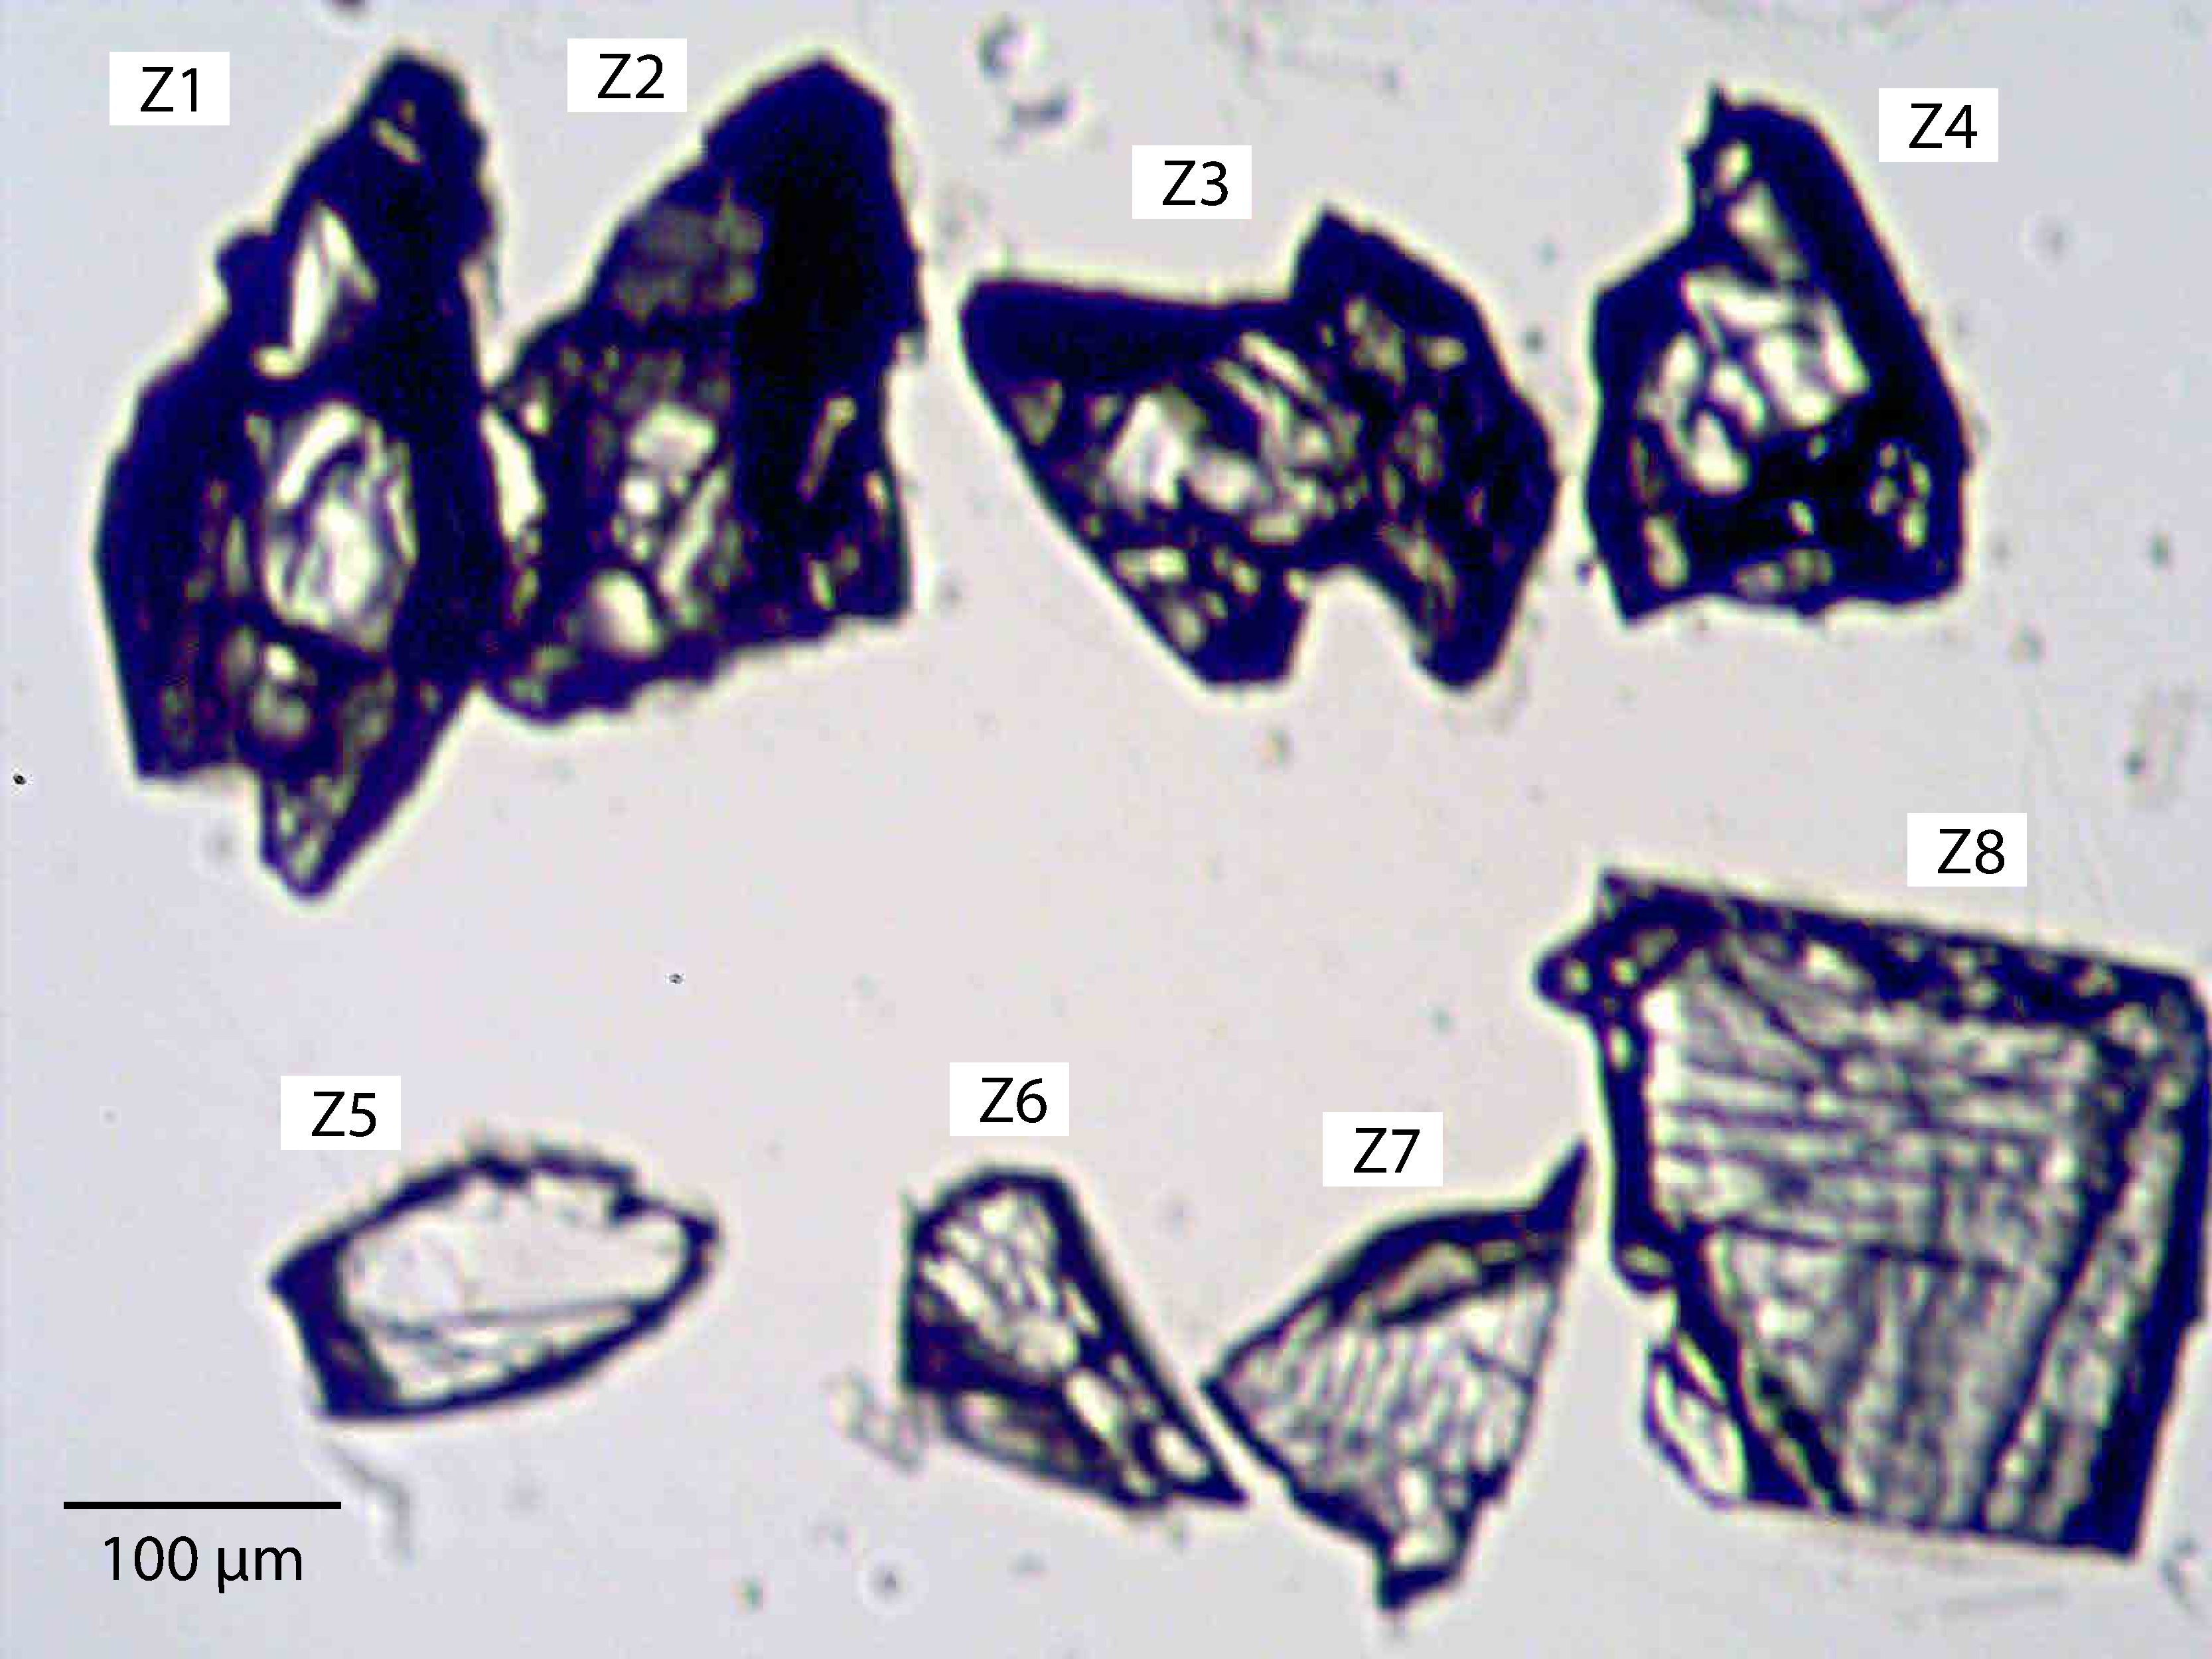
\includegraphics[width=0.8\textwidth]{Figure/SI_zircons.pdf}
\centering
\caption{\footnotesize{Image of individual zircons used for ID-TIMS U-Pb geochronology from sample MS99033. Zircons (z1-z4) are subhedral to anhedral crystals and (z5-z8) are platy fragments.}}
\label{fig:zircon_image}
\end{figure}

\begin{figure}[h!]
\noindent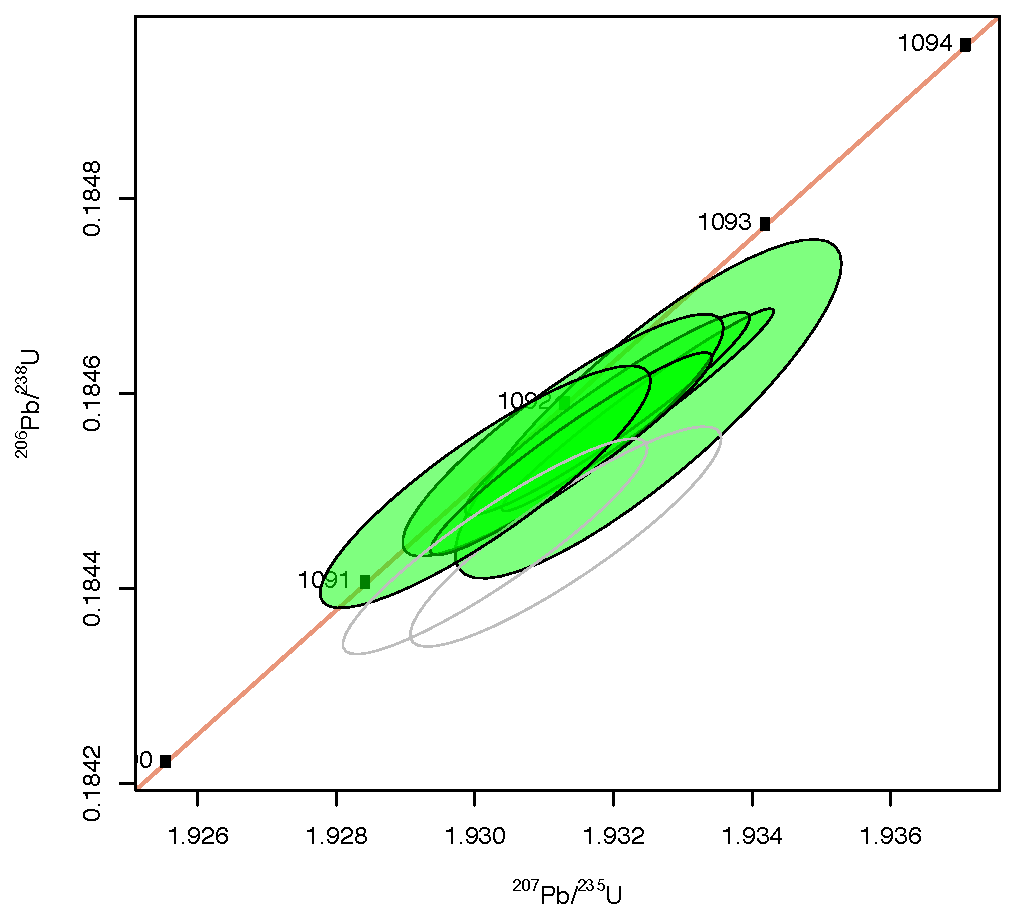
\includegraphics[width=0.8\textwidth]{Figure/SI_MS99033_geochron_plot.pdf}
\centering
\caption{\footnotesize{U-Pb concordia plots for the new zircon dates from anorthosite xenoliths AX16, geochronology sample MS99033. The ellipses represent 2$\sigma$ analytical uncertainty on individual zircon dates. Green filled ellipses are analyses included in the $^{206}$Pb/$^{238}$U weighted mean dates while the grey ellipses are those that were excluded. }}
\label{fig:zircon_concordia}
\end{figure}

U-Pb dates were obtained by chemical abrasion isotope dilution thermal ionization mass spectrometry (ID-TIMS) in the Boise State University (BSU) Isotope Geology Laboratory (Table S2; Fig. \ref{fig:zircon_image}). 

Zircons were separated from the bulk rock sample using a sledge, Retsch DM200 disc mill, 500 µm sieve, Wilfley Shaker Table, LB-1 Frantz magnetic separator, and methylene iodide heavy liquid. Heavy separates were annealed at 900\textdegree C for 48 to 60 hours in quartz crucibles in a muffle furnace. Individual zircons were chemically abraded. Chemical abrasion was carried out by transferring zircons to 3 ml Teflon Perfluoroalkoxy alkane (PFA) beakers in which they were rinsed in 3.5 M HNO$_\mathrm{3}$ and ultrapure H$_\mathrm{2}$O prior to loading into 300 $\mu$l Teflon PFA microcapsules. Fifteen microcapsules were placed in a large-capacity Parr vessel and the zircon partially dissolved in 120 $\mu$l of 29 M HF for 12 hours at 190\textdegree C. Zircons were returned to 3 ml Teflon PFA beakers, HF was removed, and zircons were immersed in 3.5 M HNO$_\mathrm{3}$, ultrasonically cleaned for an hour, and fluxed on a hotplate at 80°C for an hour. The HNO$_\mathrm{3}$ was removed and zircon was rinsed twice in ultrapure H2O before being reloaded into the 300 $\mu$l Teflon PFA microcapsules (rinsed and fluxed in 6 M HCl during sonication and washing of the zircons) and spiked with the $^{233}$U-$^{235}$U-$^{205}$Pb BSU tracer solution (BSU1B). Zircons were dissolved in Parr vessels in 120 $\mu$l of 29 M HF at 220\textdegree C for 48 hours, dried to fluorides, and re-dissolved in 6 M HCl at 180\textdegree C overnight. Pb and U were separated from the zircon matrix using an HCl-based anion-exchange chromatographic procedure \citep{Krogh1973a}, eluted together and dried with 2 $\mu$l of 0.05 N H$_\mathrm{3}$PO$_\mathrm{4}$.

Pb and U were loaded on a single outgassed Re filament in 5 $\mu$l of a silica-gel/phosphoric acid mixture \citep{Gerstenberger1997a}, and Pb and U isotopic measurements made on a GV Isoprobe-T multicollector thermal ionization mass spectrometer equipped with an ion-counting Daly detector. Pb isotopes were measured by peak-jumping all isotopes on the Daly detector for 190 cycles with a mass bias correction of 0.16 $\pm$ 0.03$\%$/a.m.u. (1$\sigma$). Transitory isobaric interferences due to high-molecular weight organics, particularly on $^{204}$Pb and $^{207}$Pb, disappeared within 30-45 cycles, while ionization efficiency averaged 104 cps/pg of each Pb isotope. Linearity (to $\geq$1.4 x 10$^6$ cps) and the associated deadtime correction of the Daly detector were determined by analysis of NBS982. Uranium was analyzed as UO$_2^+$ ions in static Faraday mode on 10$^{12}$ ohm resistors for up to 300 cycles, and corrected for isobaric interference of $^{233}$U$^{18}$O$^{16}$O on $^{235}$U$^{16}$O$^{16}$O with an $^{18}$O/$^{16}$O of 0.00206. Ionization efficiency averaged 20 mV/ng of each U isotope. U mass fractionation was corrected using the $^{233}$U/$^{235}$U ratio of the BSU1B tracer. 

\subsubsection*{LA-ICPMS plagioclase geochemistry}

Rare earth elements (REE) ICPMS analyses are done by the GeoAnalytical Lab at Washington State University. Four plagioclase crystals with minimal visible other mineral inclusions from anorthosite sample MS99033 were picked for REE analyses (Table S3). The Flux used for the fusion is di-Lithium-tetraborate (Spectromelt$^@$ A-10, EM Science, Gibbstown, NJ). Reagents are HNO$_3$ 69-70\% (Fisher ACS plus grade), HF 48-52\% (Baker ACS reagent grade), HClO$_4$ 67-71\% (Fisher Trace Metal Grade), and H$_2$O$_2$ (Baker ACS Reagent). The HF is further purified before use by sub-boiling distillation in a Teflon still.  All water used is $>$18 M deionized water from a Nanopure analytical grade water system (Barnstead/Thermolyne)

Powdered samples are mixed with an equal amount of lithium tetraborate flux (typically 2g), placed in a carbon crucible and fused at 1000\textdegree C in a muffle furnace for 30 minutes. After cooling, the resultant fusion bead is briefly ground in a carbon-steel ring mill and a 250 mg portion is weighed into a 30 ml, screw-top Teflon PFA vial for dissolution. The acid dissolution consists of a first evaporation with HNO$_3$ (2ml), HF (6 ml), and HClO$_4$ (2 ml) at 110\textdegree C. After evaporating to dryness, the sample is wetted and the sides of the vial are rinsed with a small amount of water before a second evaporation with HClO$_4$ (2 ml) at 160\textdegree C. After the second evaporation, samples are brought into solution by adding approximately 10 ml of water, 3 ml HNO$_3$, 5 drops H$_2$O$_2$, 2 drops of HF and warmed on a hot plate until a clear solution is obtained. The sample is then transferred to a clean 60 ml HDPE bottle diluted up to a final weight of 60g with deionized water.

Solutions are analyzed on an Agilent model 4500 ICPMS and are diluted an additional 10X at the time of analysis using Agilent’s Integrated Sample Introduction System (ISIS). This yields a final dilution factor of 1:4800 relative to the amount of sample fused. Instrumental drift is corrected using Ru, In, and Re as internal standards. Internal standardization for the REEs uses a linear interpolation between In and Re after \cite{Doherty1989a} to compensate for mass-dependant differences in the rate and degree of instrumental drift. Isobaric interference of light rare earth oxides on the mid- heavy REEs can be a significant source of error in ICPMS analysis, so tuning is optimized to keep the CeO/Ce ratio below 0.5\%. Correction factors used to compensate for the remaining oxide interferences are estimated using two mixed-element solutions. The first contains Ba, Pr, and Nd, and the second Tb, Sm, Eu, and Gd.  Standardization is accomplished by processing duplicates of three in-house rock standards interspersed within each batch of 18 unknowns. Concentrations, oxide- and drift corrections are then calculated offline using a spreadsheet. Methods description is provided by: \url{https://environment.wsu.edu/facilities/geoanalytical-lab/technical-notes/icp-ms-method/}.  


\subsubsection*{LA-ICPMS zircon geochemistry}

% \begin{figure}[h!]
% \noindent\includegraphics[width=0.7\textwidth]{Figure/SI_REE.pdf}
% \centering
% \caption{\footnotesize{Top: Rare earth element (REE) analyses on anorthosite xenoliths and plagioclase crystals by \cite{Morrison1983a}; Bottom: REE analyses on 15 zircons from geochronology sample MS99033 via inductively coupled plasma mass spectrometry. }}
% \label{fig:REE}
% \end{figure}

15 zircons extracted from sample MS99033 were analyzed by laser ablation inductively coupled plasma mass spectrometry (LA-ICPMS) using a ThermoElectron, iCAP-RQ, single quadrupole ICPMS and a Teledyne (Photon Machines) Analyte Excite+ 193 nm excimer Analyte laser with a HelEx ablation cell at BSU. Analytical protocols, standard materials, and data reduction software developed at BSU were used for acquisition and calibration of U-Pb dates and a suite of high field strength elements (HFSE) and rare earth elements (REE). Zircon were ablated with a 25 µm diameter laser spot using fluence and pulse rates of $\sim$2.5 J/cm2 and $\sim$5 Hz, respectively, during a 20-second analysis excavating a pit 25 µm deep. Ablated material was carried to the nebulizer flow of the plasma by a 1.2 L/min He gas stream. Total sweep duration is 895 ms, and quadrupole dwell times were 5 ms for Si and Zr, 40 ms for $^{202}$Hg, $^{204}$Pb, $^{208}$Pb, $^{232}$Th, and $^{238}$U, 80 ms for $^{206}$Pb, 200 ms for $^{49}$Ti and $^{207}$Pb, and 10 ms for all other HFSE and REE. Background count rates were obtained prior to each spot analysis and subtracted from the raw count rate for each analyte. Concentrations were calculated using background-subtracted count rates internally normalized to $^{29}$Si and calibrated with the primary standards NIST SRM-610 and -612 glasses. Ablation pits that intersected mineral inclusions were identified based on Ti and P spikes. The Ti-in-zircon thermometer was calculated using an average TiO$_2$ activity value of 0.7 in crustal rocks \citep{Watson2006a} and an average SiO$_2$ activity value of 1.0 \citep{Ferry2007a}. 

% \begin{figure}[h!]
% \noindent\includegraphics[width=0.7\textwidth]{Figure/SI_CL_montage.pdf}
% \centering
% \caption{\footnotesize{Cathodoluminescnece (CL) image montage of the 15 laser-ablated zircons. Immediately apparent are sharp boundaries between zones of differing CL response within many crystals. The bright zoning in grain 15 has a thickness of $\sim$2 $\mu$m. Note that grain 1 (corresponding to spot 1) has a platy morphology, while the rest are subhedral to anhedral zircons. }}
% \label{fig:CL_image}
% \end{figure}

%For U-Pb and $^{207}$Pb/$^{206}$Pb dates, instrumental fractionation of the background-subtracted ratios was corrected and dates were calibrated with respect to interspersed measurements of standards and reference materials. The primary zircon standard Ple\v{s}ovice \citep{Slama2008a} was used to monitor time-dependent instrumental fractionation based on two for every 10 analyses of unknown zircons. Secondary standards were also analysed twice for every 10 unknowns, and a secondary correction was applied to the 206Pb/238U dates using Seiland (~530 Ma) and FC1 (~1099 Ma). Radiogenic isotope ratio and age error propagation for all analyses includes uncertainty contributions from counting statistics and background subtraction. These uncertainties are the local standard deviations of the polynomial fits to the interspersed primary standard measurements versus time for the time-dependent, relatively larger U-Pb fractionation factor, and the standard errors of the means of the consistently time-invariant and smaller $^{207}$Pb/$^{206}$Pb fractionation factor. These uncertainties are 1.00–2.10\% (average of ~1.5\%) (2 sigma) for $^{206}$Pb/$^{238}$U and 0.22–1.03\% (average of $\sim$0.6\%) (2 sigma) for $^{207}$Pb/$^{206}$Pb. Errors on dates from individual analyses are given at 2 sigma (Table DR2), and errors on weighted mean dates include the standard calibration uncertainties within each experiment and are also given at 2 sigma.

% The resulting zircon REE diagrams are shown in Fig. \ref{fig:REE}. All zircons analyzed show a strong negative Eu anomaly on chondrite-normalized REE diagrams \citep{Sun1989a}. This result is consistent with the zircons having crystallized from a liquid that has had significant plagioclase extraction. On the other hand, REE analyses on anorthosite xenoliths whole rocks and plagioclase crystals from \citep{Morrison1983a} show positive Eu anomaly. The opposite Eu anomalies from plagioclase and zircons allow for an interpretation that they crystallized from the same parent magma. The cathodoluminescence images of the 15 laser-ablated zircons are shown in Fig. \ref{fig:CL_image}. 

\subsubsection*{Additional zircon photomicrograph}
\begin{figure}[h!]
\noindent\includegraphics[width=\textwidth]{Figure/SI_interstitial_zircons.pdf}
\caption{\footnotesize{Back scattered electron (BSE) images of anorthosite xenoliths. Subhedral to anhedral zircons form next to mafic melt pockets.}}
\label{fig:interstitial_zircons}
\end{figure}

Fig. \ref{fig:interstitial_zircons} shows subhedral and anhedral zircons in anorthosite xenoliths AX11 and AX 21 in back scattered electron (BSE) images of anorthosite thin sections. All zircons found are interstitial to the plagioclase. This texture is consistent with the interpretation of a zircon formation from interstitial melt liquids preserved in plagioclase mush.

% \subsubsection*{Evaluating Pb diffusive loss}

% Our thermal history modeling indicates that the xenoliths could have equilibrated to the temperature of the olivine tholeiitic magma ($\sim$1100 to 1200\textdegree C) and remained at that temperature for more than 100 years in the diabase sill interior. Following the Pb diffusion rate from \cite{Cherniak2001a}, we plotted the temperature and time relationships for diffusing out Pb from zircons with effective radii of 60 $\mu$m in Fig. \ref{fig:diffusive_loss}. The model shows that if a temperature of 1200\textdegree C is sustained for $\sim$10 thousand years (before the final cooling after diabase emplacement), $\sim$90\% of Pb will diffuse out of a $\sim$120 $\mu$m diameter zircon. Assuming that the zircons from MS99033 crystallized at 1096 Ma and suffered various degrees of Pb loss ranging from 90\% to 99\% at 1091.6 Ma, they could give apparent U-Pb dates of 1091.8 Ma (Fig. \ref{fig:diffusive_loss}). However, if the zircons crystallized in the Paleoproterozoic and experienced the same percentage range of Pb loss, discordant U-Pb dates with much older ages than is observed would be expected (Fig. \ref{fig:diffusive_loss}).

% Therefore, based on the U-Pb systematics alone we cannot rule out the scenario where the Beaver River anorthosite xenoliths crystallized during the Duluth Complex time. However, re-equilibration of Dy elemental zoning throughout zircon grains is expected if 90\% Pb loss occurred. Given that our CL images show sharp boundaries between bright and dark zones which are dominantly attributed to the variation in Dy concentrations, it is unlikely that the zircons from anorthosite AX16 experienced such prolonged heating and associated high percentages of Pb loss after initial crystallization. 

% \begin{figure}[h!]
% \noindent\includegraphics[width=0.55\textwidth]{Figure/SI_diffusive_loss.pdf}
% \centering
% \caption{\footnotesize{Top: Conditions for diffusive Pb loss in crystalline zircon for zircons of effective radii of 60 $\mu$m. Curves represent time–temperature conditions under which zircon will lose the indicated fraction of total Pb; Middle: Modeled zircon Pb loss scenarios with initial crystallization of 1091.8 Ma, 1096 Ma, and 1800 Ma ages with varying degrees of Pb loss at 1091.6 Ma compared to the actual U-Pb dates; Bottom: Preservation of Dy zoning in zircon. Curves represent time-temperature conditions under which different zoning thicknesses would be preserved in zircon. For conditions above the upper solid curves in each group, well-defined zoning will be lost. For conditions above the dashdot lines zones will be partially lost but still retain initial composition in zone center. Pb diffusion and Dy zoning models are replotted from \cite{Cherniak1997a}.}}
% \label{fig:diffusive_loss}
% \end{figure}


\subsubsection*{Beaver River diabase structural correction}

Structural measurements were obtained from the published geologic maps of the study area as well as our field data. We calculated the mean directions from the combined volcanic bedding measurements from the Schroeder-Lutsen basalt and igneous layering measurements from the Beaver River diabase and constructed two sets of tilt correction data for the paleomagnetic sites in the southern and eastern Beaver Bay Complex \citep{Boerboom2004a, Boerboom2006a, Boerboom2006b, Boerboom2007a, Miller2001a}. The mean dip angle for the two areas are very similar while the dip trends are different, with the southern Beaver Bay Complex showing a slightly more easterly trend than the eastern Beaver Bay Complex. This difference in dip trend reflects the overall arcuate shape of the Beaver Bay Complex intrusions along the shore of Lake Superior. 

\begin{figure}[h!]
\noindent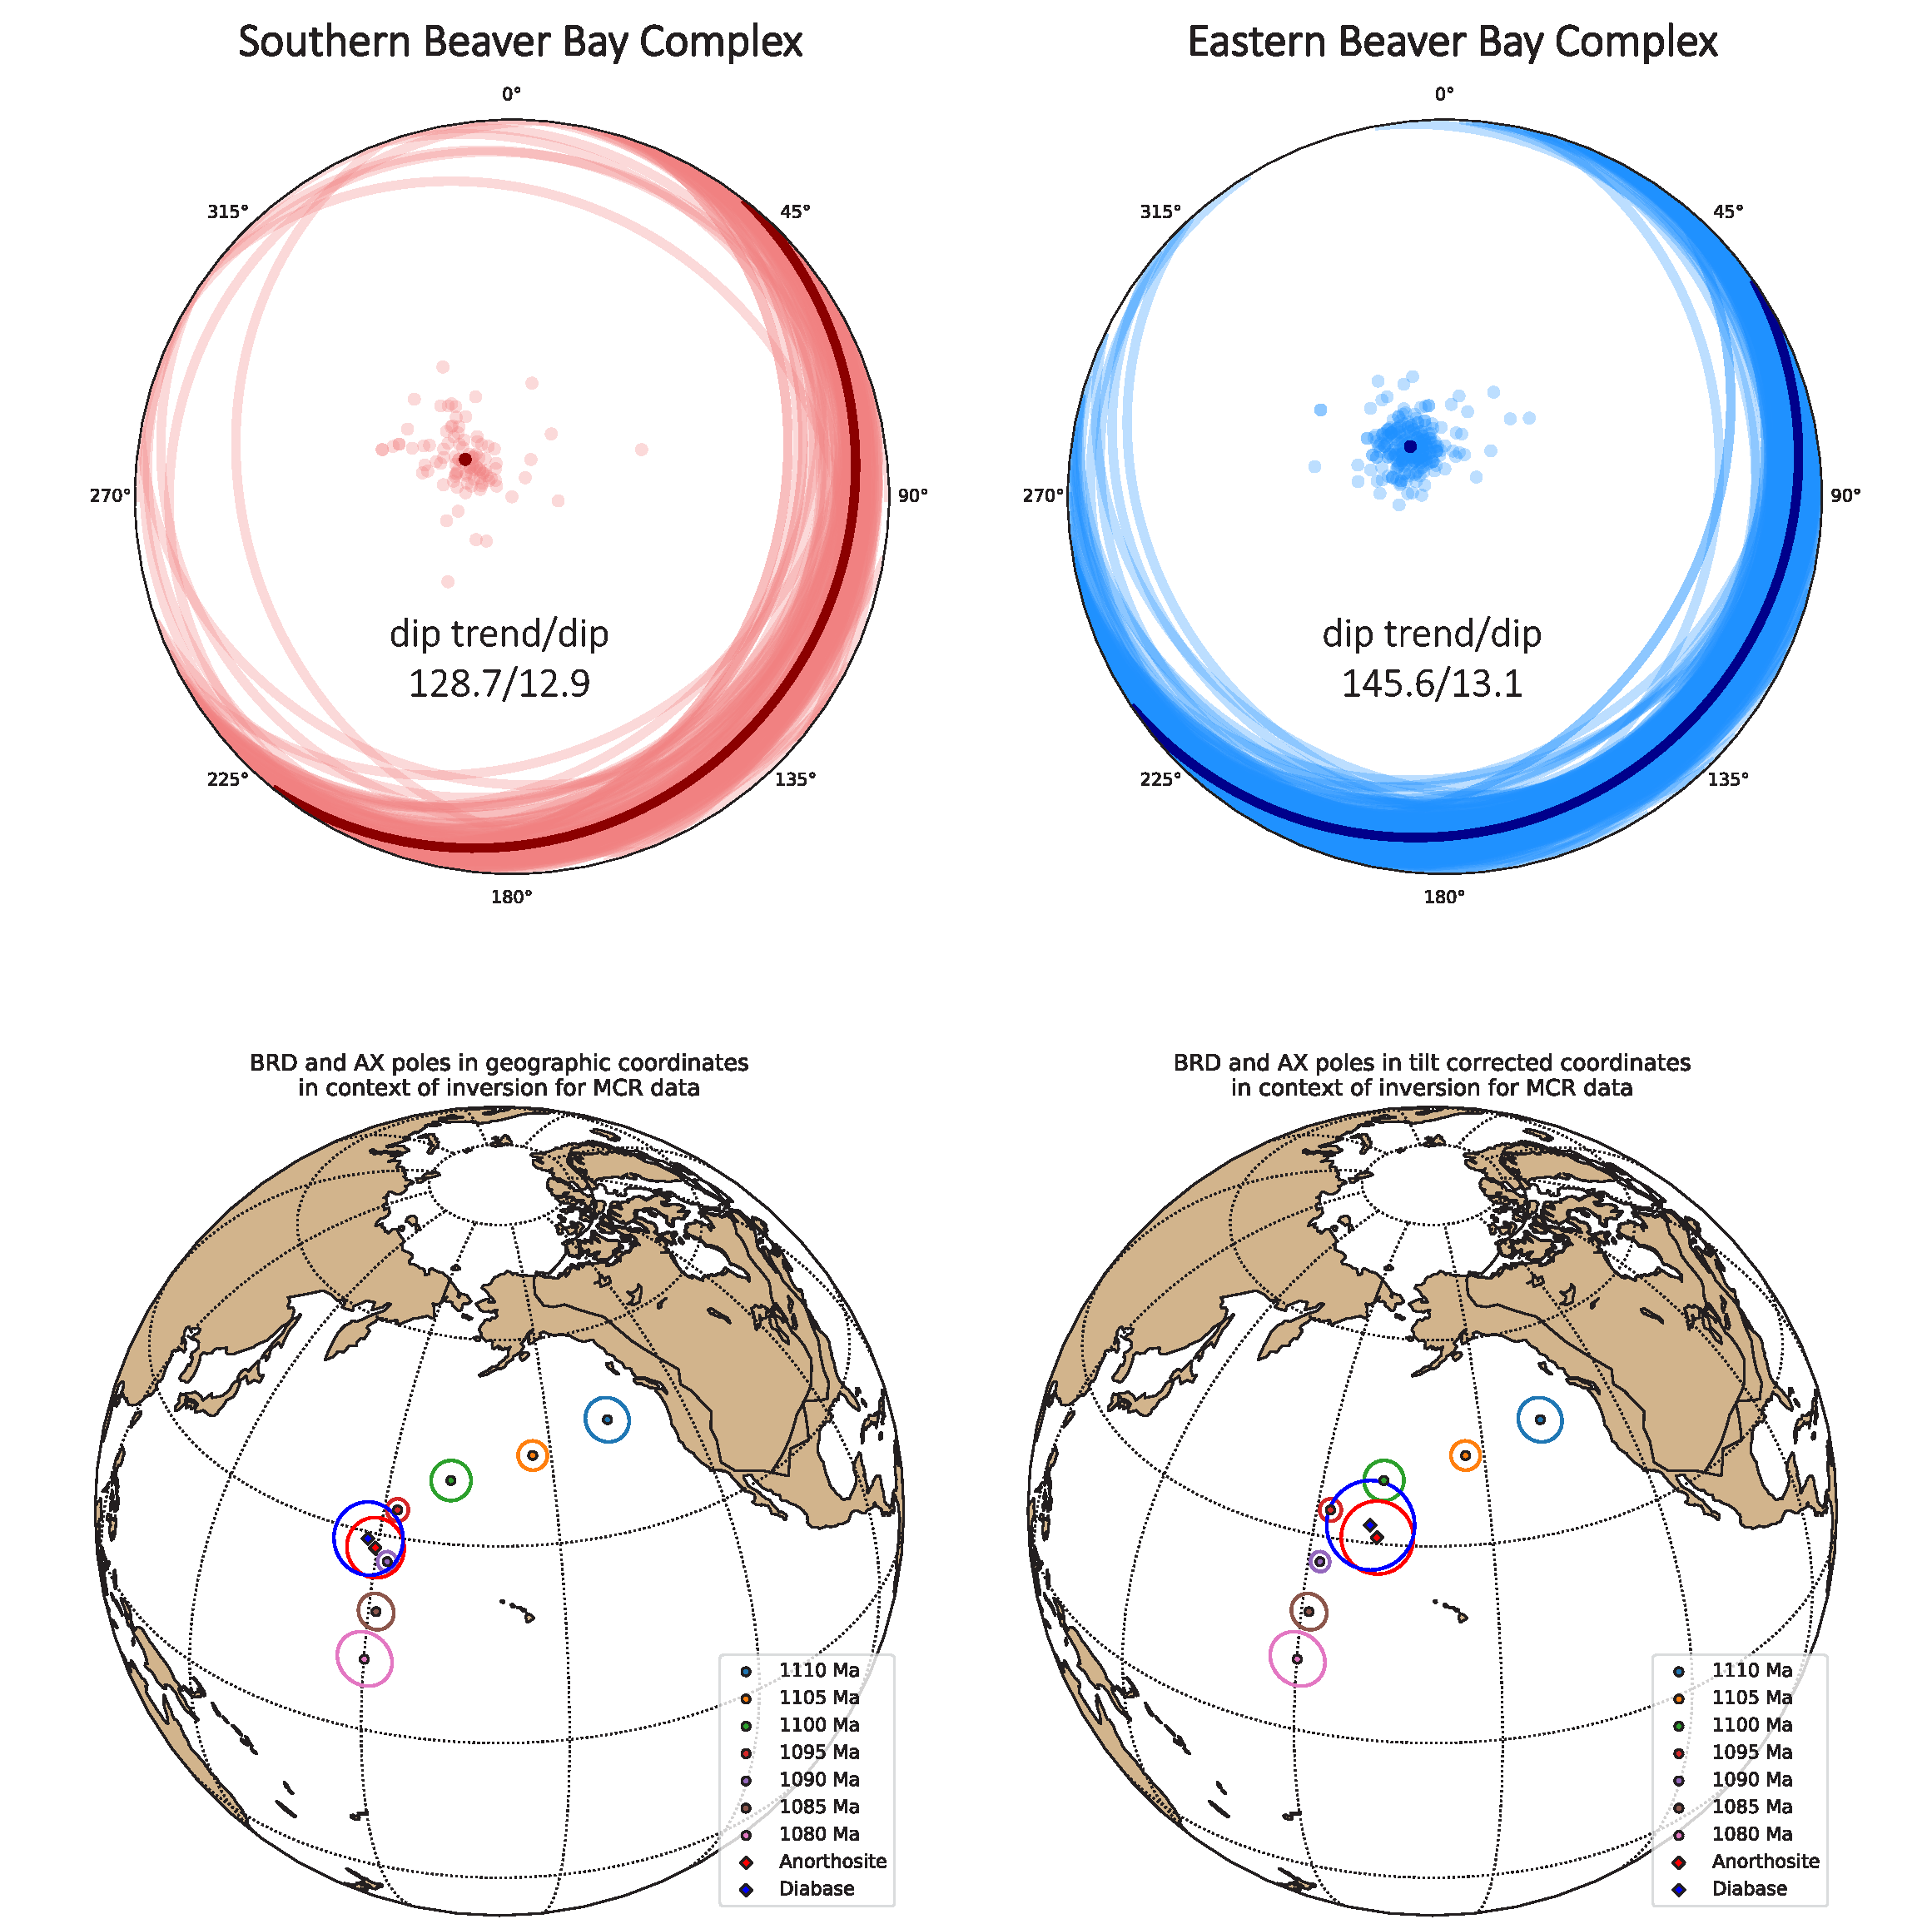
\includegraphics[width=0.8\textwidth]{Figure/SI_tilt_correction.pdf}
\centering
\caption{\footnotesize{Stereonet plots of the compiled structural orientation data to tilt correct the paleomagnetic directions obtained from the Beaver River diabase and the anorthosite xenoliths therein. The mean pole position of the diabase and anorthosite units before and after the tilt correction are shown in context of the inverted Keweenawan Track developed by \cite{Swanson-Hysell2019a}.}}
\label{fig:tilt_correction}
\end{figure}

To summarize, We use a bedding dip direction - dip of 145.6 - 13.1 for paleomagnetic site AX3, AX4, AX5, AX6, AX7, AX8, AX9, AX10, and BD2, BD14, BD15, BD16 in the Eastern Beaver Bay Complex region. We use a bedding dip direction - dip of 128.7 - 12.9 for site AX1, AX2, AX11, AX12, AX13, AX14, AX15, AX16, AX17, AX18, AX19, AX20, AX21, AX22, BD1, BD3, BD4, BD5, BD6, BD7. BD8. BD9, BD10, BD11, BD12, BD13, BD17 in the Southern Beaver Bay Complex.

Fig. \ref{fig:tilt_correction} shows the stereonet plots of the bedding orientations compiled for tilt correcting the paleomagnetic directions of samples collected in the Southern Beaver Bay Complex and the Eastern Beaver Bay Complex. The resultant mean pole position for the diabase changes from 29.0\textdegree N, 178.2\textdegree E, N = 15, A95 = 5.2, k = 55.3 before tilt correction to 32.5\textdegree N, 189.5\textdegree E, N = 15, A95 = 6.3, k = 37.4 after tilt correction. For the anorthosite, the mean pole position changes from 28.0\textdegree N, 179.6\textdegree E, N = 17, A95 = 4.3, k = 70.6 before tilt correction to 30.9\textdegree N, 190.8\textdegree E, N = 17, A95: 5.2, k = 48.5 after tilt correction. The uncertainty ellipses for both units are slightly larger after tilt correcting the directions. This may reflect the uncertainties associated with using igneous fabrics as our paleohorizontal references. Nevertheless, the mean pole position of the diabase and anorthosite still overlaps and is consistent with the expected position derived from the inverted Keweenawan Track \textit{ca.} 1092 Ma \citep{Swanson-Hysell2019a}. 


\clearpage
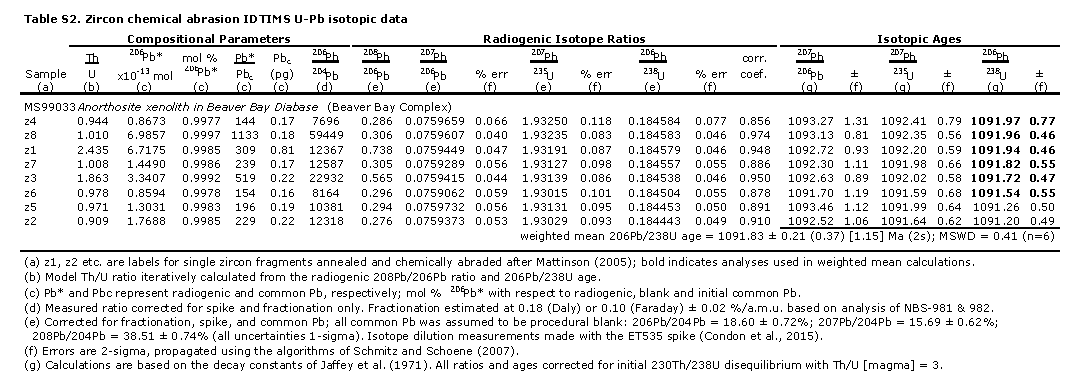
\includepdf[pages=-,pagecommand={},width=7.65 in]{Figure/SI_MS99033_geochron.pdf}

\clearpage
\includepdf[pages=-,pagecommand={},width=7.65 in]{Figure/SI_plag_REE_table.pdf}


\clearpage

% \small
% \begin{thebibliography}{6}
% \providecommand{\natexlab}[1]{#1}
% \providecommand{\url}[1]{\texttt{#1}}
% \providecommand{\urlprefix}{URL }
% \expandafter\ifx\csname urlstyle\endcsname\relax
%   \providecommand{\doi}[1]{doi:\discretionary{}{}{}#1}\else
%   \providecommand{\doi}{doi:\discretionary{}{}{}\begingroup
%   \urlstyle{rm}\Url}\fi

% \bibitem[{Boerboom (2004)}]{Boerboom2004a}
% Boerboom, T. J., 2004. {M-147 Bedrock geology of the Split Rock Point quadrangle, Lake County, Minnesota(Tech. Rep.)}. Minnesota Geological Survey.

% \bibitem[{Boerboom and Green (2006)}]{Boerboom2006a}
% Boerboom, T. J., \& Green, J. C., 2006. {M-170 Bedrock geology of the Schroeder quadrangle, Cook County, Minnesota(Tech. Rep.)}. Minnesota Geological Survey.

% \bibitem[{Boerboom et al. (2006)}]{Boerboom2006b}
% Boerboom, T. J., Green, J. C., Albers, P., \& Miller, J., J.D, 2006. {M-171 bedrock geology of the tofte quadrangle, cook county, minnesota(Tech. Rep.)}. Minnesota Geological Survey.

% \bibitem[{Boerboom et al. (2007)}]{Boerboom2007a}
% Boerboom, T. J., Green, J., \& Albers, P., 2007. {M-174 Bedrock geology of the Lutsen quadrangle, Cook County, Minnesota(Tech. Rep.)}. Minnesota Geological Survey.

% \bibitem[{Cherniak and Watson (2001)}]{Cherniak2001a}
% Cherniak, D. J., \& Watson, E. B., 2001. {Pb diffusion in zircon}. Chemical Geology, 172(1-2), 5-24, \doi{10.1016/s0009-2541(00)00233-3}.

% \bibitem[{Doyle (2016)}]{Doyle2016a}
% Doyle, M., 2016. {Geologic and geochemical attributes of the Beaver River Diabase and Greenstone Flow: Testing a possible intrusive-volcanic link in the 1.1 Ga Midcontinent Rift}. (Unpublished master’s thesis). University of Minnesota.

% \bibitem[{Gerstenberger and Haase(1997)}]{Gerstenberger1997a}
% Gerstenberger, H. and Haase, G., 1997. {A highly effective emitter substance for mass spectrometric {P}b isotope ratio determinations}. Chemical Geology, vol. 136, pp. 309--312.

% \bibitem[{Hiess et~al.(2012)Hiess, Condon, McLean, and Noble}]{Hiess2012a}
% Hiess, J., Condon, D.~J., McLean, N., and Noble, S.~R., 2012. {$^{238}${U}/$^{235}${U} systematics in terrestrial uranium-bearing minerals} Science, vol. 335, pp. 1610--1614, \doi{10.1126/science.1215507}.

% \bibitem[{Krogh(1973)}]{Krogh1973a}
% Krogh, T., 1973, A low contamination method for the hydrothermal decomposition of zircon and extraction of {U} and {P}b for isotopic age determinations: Geochimica Cosmochimicha Acta, vol.~37, pp. 485--494, \doi{10.1016/0016-7037(73)90213-5}.

% \bibitem[{Ludwig(2003)}]{Ludwig2003a}
% Ludwig, K.~R., 2003, Isoplot 3.0. a geochronological toolkit for {M}icrosoft {E}xcel: Tech. rep., Berkeley Geochronology Center.

% \bibitem[{Mattinson(2005)}]{Mattinson2005a}
% Mattinson, J.~M., 2005, {Zircon U/Pb chemical abrasion (CA-TIMS) method:
%   Combined annealing and multi-step partial dissolution analysis for improved
%   precision and accuracy of zircon ages}: Chemical Geology, vol. 220, pp.
%   47--66, \doi{10.1016/j.chemgeo.2005.03.011}.

% \bibitem[{Miller et al.(2006)}]{Miller2001a}
% Miller Jr, J. D., Severson, M. J., Chandler, V. W., \& Peterson, D. M., 2001. {M-119651Geologic map of the Duluth Complex and related rocks, northeastern Minnesota652(Tech. Rep.)}.  Minnesota Geological Survey. 

% \bibitem[{Morrison et al.(1983)}]{Morrison1983a}
% Morrison, D. A., Ashwal, L. D., Phinney, W. C., Shih, C. Y., \& Wooden, J. L., 1983. {Pre-Keweenawan anorthosite inclusions in the Keweenawan Beaver Bay and Duluth complexes, northeastern Minnesota}. Geological Society of America Bulletin, 94(2), 206-221, \doi{10.1130/0016-7606(1983)94<206:paiitk>2.0.co;2}.

% \bibitem[{Paces and Miller (1993)}]{Paces1993a}
% Paces, J. B., and Miller Jr, J. D., 1993. {Precise U‐Pb ages of Duluth complex and related mafic intrusions, northeastern Minnesota: Geochronological insights to physical, petrogenetic, paleomagnetic, and tectonomagmatic processes associated with the 1.1 Ga Midcontinent Rift system}. Journal of Geophysical Research: Solid Earth, 98(B8), 13997-14013, \doi{10.1029/93jb01159}.

% % \bibitem[{Pedersen, Dunning, & Robins 1989}]{Pedersen1989a}
% % Pedersen, R. B., Dunning, G. R., & Robins, B., 1989. {U-Pb ages of nepheline syenite pegmatites from the Seiland Magmatic Province, N. Norway. In The Caledonides geology of Scandinavia}. Conference dedicated to the Memory of Dr Sven Foyn (pp. 3-8). 

% \bibitem[{Schmitz and Schoene (2007)}]{Schmitz2007b}
% Schmitz, M.~D. and Schoene, B., 2007. {Derivation of isotope ratios, errors,
%   and error correlations for U-Pb geochronology using
%   $^{205}$Pb-$^{235}$U-($^{233}$U)-spiked isotope dilution thermal ionization
%   mass spectrometric data}. Geochem. Geophys. Geosyst., vol.~8, p. Q08,006,
%   \doi{10.1029/2006GC001492}.

% \bibitem[{Slama et al.(2008)}]{Slama2008a}
% Sláma, J., Košler, J., Condon, D. J., Crowley, J. L., Gerdes, A., Hanchar, J. M., ... \& Whitehouse, M. J., 2008. {Ple{\v{s}}ovice zircon—a new natural reference material for U–Pb and Hf isotopic microanalysis}. Chemical Geology, 249(1-2), 1-35, \doi{10.1016/j.chemgeo.2007.11.005}.

% \bibitem[{Sun and McDonough (1989)}]{Sun1989a}
% Sun, S. S., \& McDonough, W. F., 1989. {Chemical and isotopic systematics of oceanic basalts: implications for mantle composition and processes}. Geological Society, London, Special Publications, 42(1), 313-345, \doi{10.1144/gsl.sp.1989.042.01.19}.

% \bibitem[{Watson et al.(2006)}]{Watson2006a}
% Watson, E. B., Wark, D. A., and Thomas, J. B., 2006. {Crystallization thermometers for zircon and rutile}. Contributions to Mineralogy and Petrology, 151(4), 413, \doi{10.1007/s00410-006-0068-5}.

% % \bibitem[{Schoene & Bowring (2007}]{Schoene2007a}
% % Schoene, B., & Bowring, S. A., 2007. {Determining accurate temperature–time paths from U–Pb thermochronology: An example from the Kaapvaal craton, southern Africa}. Geochimica et Cosmochimica Acta, 71(1), 165-185, \doi{10.1016/j.gca.2006.08.029}.

% \end{thebibliography}

\bibliographystyle{gsabull}
\bibliography{YZ_ref}

\end{document}

